% Specify document class
\documentclass[12pt,a4paper]{article}
% Load packages
\usepackage[utf8]{inputenc}
\usepackage{amsmath}
\usepackage{amsfonts}
\usepackage{amssymb}
\usepackage{graphicx}
\usepackage{listings}
\usepackage{float}

% Define author name and title of document
\author{Hannah Frank}
\title{Analysis of Movie Genre and Ratings}

\begin{document} % Begin document

\maketitle % Creates title, including date
	
\section{Research Question} % Begin chapter
Do different genres receive varying critical appreciation? We compare 3 movie genres (`Comedy', `Documentary', `Drama') with their ratings (`Rotten', `Fresh', `Certified Fresh') to determine if there is a statistically significant correlation between the two variables.

\section{Analysis}
The tables below provide the joint distribution of raw values (Figure \ref{tab:tab}) and conditional distributions of proportions (Table \ref{tab:prob_tab}). The  conditional distributions in Table \ref{tab:prob_tab}  show non-identical distributions of ratings according to genre. The probability of ``Rotten'' conditional on the movie being a comedy is ...., while the probability of ``Rotten'' conditional on the movie being a documentary is only.... This is a first indication that genre and ratings are not independent. 
	
\begin{figure}[H] % Begin figure and verbatim environment which allows to input R code and R output
\begin{verbatim} 
	                    critics_rating
	genre                Rotten Fresh Certified Fresh
	Comedy                 63    14              10
	Documentary             3    32              17
	Drama                 124   106              75
\end{verbatim}
\caption{Contingency table--Joint distribution raw values}
\label{tab:tab}
\end{figure}

\begin{table}[H] % Alternatively, we can use the table environment in Latex
\centering
\begin{tabular}{lcccc} 
\hline
Genre/rating & Rotten & Fresh & Certified Fresh & Sum \\ 
\hline
Comedy & 0.72 & 0.16 & 0.11 &1.0 \\ 
Documentary & 0.06 & 0.62 &  0.33 & 1.0 \\
Drama & 0.41 & 0.35 & 0.25 &1.0 \\
\hline
\end{tabular}
\caption{Contingency table--Conditional distributions proportions}
\label{tab:prob_tab}
\end{table}

We also visualize the results in Table \ref{tab:prob_tab} in Figure \ref{fig:barplot}, which  confirms that the probability of ``Rotten'' varies greatly depending on the genre. 

\begin{figure}[H] % Place figure here
\centering
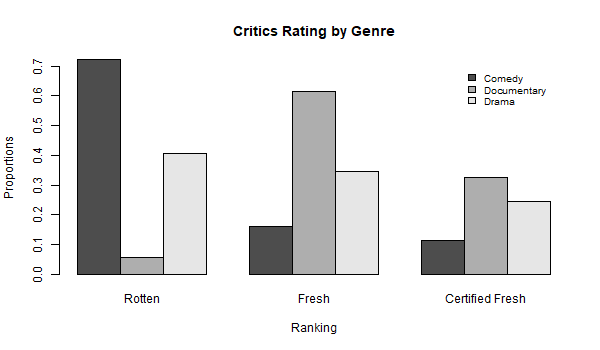
\includegraphics[scale=0.5]{barplot.png}
\caption{Bar plot--Conditional distributions proportions}
\label{fig:barplot}
\end{figure} 

Finally, we us the Chi-square test of independence to validate whether genre and ratings are independent or not. The code used is detailed below:

\begin{verbatim}
# Run Chi squared test
chisq.test(df_s$genre, df_s$critics_rating)
\end{verbatim}

The results of the test were as follows:

\begin{verbatim}
Pearson's Chi-squared test

data:  df_s$genre and df_s$critics_rating
X-squared = 62.008, df = 4, p-value = 1.097e-12
\end{verbatim}

\section{Conclusion}

In conclusion, we rejected the null hypothesis that ranking and genre are  independent. In particular, we note that Comedy seems to be more likely to receive rotten reviews, while documentaries are less likely to receive rotten reviews. 

\end{document} % End document